% Options for packages loaded elsewhere
\PassOptionsToPackage{unicode}{hyperref}
\PassOptionsToPackage{hyphens}{url}
\PassOptionsToPackage{dvipsnames,svgnames,x11names}{xcolor}
%
\documentclass[
]{article}
\title{Ejercicios Tema 2 - Variables aleatorias}
\author{Ricardo Alberich, Juan Gabriel Gomila y Arnau Mir}
\date{Curso de Probabilidad y Variables Aleatorias con R y Python}

\usepackage{amsmath,amssymb}
\usepackage{lmodern}
\usepackage{iftex}
\ifPDFTeX
  \usepackage[T1]{fontenc}
  \usepackage[utf8]{inputenc}
  \usepackage{textcomp} % provide euro and other symbols
\else % if luatex or xetex
  \usepackage{unicode-math}
  \defaultfontfeatures{Scale=MatchLowercase}
  \defaultfontfeatures[\rmfamily]{Ligatures=TeX,Scale=1}
\fi
% Use upquote if available, for straight quotes in verbatim environments
\IfFileExists{upquote.sty}{\usepackage{upquote}}{}
\IfFileExists{microtype.sty}{% use microtype if available
  \usepackage[]{microtype}
  \UseMicrotypeSet[protrusion]{basicmath} % disable protrusion for tt fonts
}{}
\makeatletter
\@ifundefined{KOMAClassName}{% if non-KOMA class
  \IfFileExists{parskip.sty}{%
    \usepackage{parskip}
  }{% else
    \setlength{\parindent}{0pt}
    \setlength{\parskip}{6pt plus 2pt minus 1pt}}
}{% if KOMA class
  \KOMAoptions{parskip=half}}
\makeatother
\usepackage{xcolor}
\IfFileExists{xurl.sty}{\usepackage{xurl}}{} % add URL line breaks if available
\IfFileExists{bookmark.sty}{\usepackage{bookmark}}{\usepackage{hyperref}}
\hypersetup{
  pdftitle={Ejercicios Tema 2 - Variables aleatorias},
  pdfauthor={Ricardo Alberich, Juan Gabriel Gomila y Arnau Mir},
  colorlinks=true,
  linkcolor={Maroon},
  filecolor={Maroon},
  citecolor={Blue},
  urlcolor={Blue},
  pdfcreator={LaTeX via pandoc}}
\urlstyle{same} % disable monospaced font for URLs
\usepackage[margin=1in]{geometry}
\usepackage{color}
\usepackage{fancyvrb}
\newcommand{\VerbBar}{|}
\newcommand{\VERB}{\Verb[commandchars=\\\{\}]}
\DefineVerbatimEnvironment{Highlighting}{Verbatim}{commandchars=\\\{\}}
% Add ',fontsize=\small' for more characters per line
\usepackage{framed}
\definecolor{shadecolor}{RGB}{248,248,248}
\newenvironment{Shaded}{\begin{snugshade}}{\end{snugshade}}
\newcommand{\AlertTok}[1]{\textcolor[rgb]{0.94,0.16,0.16}{#1}}
\newcommand{\AnnotationTok}[1]{\textcolor[rgb]{0.56,0.35,0.01}{\textbf{\textit{#1}}}}
\newcommand{\AttributeTok}[1]{\textcolor[rgb]{0.77,0.63,0.00}{#1}}
\newcommand{\BaseNTok}[1]{\textcolor[rgb]{0.00,0.00,0.81}{#1}}
\newcommand{\BuiltInTok}[1]{#1}
\newcommand{\CharTok}[1]{\textcolor[rgb]{0.31,0.60,0.02}{#1}}
\newcommand{\CommentTok}[1]{\textcolor[rgb]{0.56,0.35,0.01}{\textit{#1}}}
\newcommand{\CommentVarTok}[1]{\textcolor[rgb]{0.56,0.35,0.01}{\textbf{\textit{#1}}}}
\newcommand{\ConstantTok}[1]{\textcolor[rgb]{0.00,0.00,0.00}{#1}}
\newcommand{\ControlFlowTok}[1]{\textcolor[rgb]{0.13,0.29,0.53}{\textbf{#1}}}
\newcommand{\DataTypeTok}[1]{\textcolor[rgb]{0.13,0.29,0.53}{#1}}
\newcommand{\DecValTok}[1]{\textcolor[rgb]{0.00,0.00,0.81}{#1}}
\newcommand{\DocumentationTok}[1]{\textcolor[rgb]{0.56,0.35,0.01}{\textbf{\textit{#1}}}}
\newcommand{\ErrorTok}[1]{\textcolor[rgb]{0.64,0.00,0.00}{\textbf{#1}}}
\newcommand{\ExtensionTok}[1]{#1}
\newcommand{\FloatTok}[1]{\textcolor[rgb]{0.00,0.00,0.81}{#1}}
\newcommand{\FunctionTok}[1]{\textcolor[rgb]{0.00,0.00,0.00}{#1}}
\newcommand{\ImportTok}[1]{#1}
\newcommand{\InformationTok}[1]{\textcolor[rgb]{0.56,0.35,0.01}{\textbf{\textit{#1}}}}
\newcommand{\KeywordTok}[1]{\textcolor[rgb]{0.13,0.29,0.53}{\textbf{#1}}}
\newcommand{\NormalTok}[1]{#1}
\newcommand{\OperatorTok}[1]{\textcolor[rgb]{0.81,0.36,0.00}{\textbf{#1}}}
\newcommand{\OtherTok}[1]{\textcolor[rgb]{0.56,0.35,0.01}{#1}}
\newcommand{\PreprocessorTok}[1]{\textcolor[rgb]{0.56,0.35,0.01}{\textit{#1}}}
\newcommand{\RegionMarkerTok}[1]{#1}
\newcommand{\SpecialCharTok}[1]{\textcolor[rgb]{0.00,0.00,0.00}{#1}}
\newcommand{\SpecialStringTok}[1]{\textcolor[rgb]{0.31,0.60,0.02}{#1}}
\newcommand{\StringTok}[1]{\textcolor[rgb]{0.31,0.60,0.02}{#1}}
\newcommand{\VariableTok}[1]{\textcolor[rgb]{0.00,0.00,0.00}{#1}}
\newcommand{\VerbatimStringTok}[1]{\textcolor[rgb]{0.31,0.60,0.02}{#1}}
\newcommand{\WarningTok}[1]{\textcolor[rgb]{0.56,0.35,0.01}{\textbf{\textit{#1}}}}
\usepackage{graphicx}
\makeatletter
\def\maxwidth{\ifdim\Gin@nat@width>\linewidth\linewidth\else\Gin@nat@width\fi}
\def\maxheight{\ifdim\Gin@nat@height>\textheight\textheight\else\Gin@nat@height\fi}
\makeatother
% Scale images if necessary, so that they will not overflow the page
% margins by default, and it is still possible to overwrite the defaults
% using explicit options in \includegraphics[width, height, ...]{}
\setkeys{Gin}{width=\maxwidth,height=\maxheight,keepaspectratio}
% Set default figure placement to htbp
\makeatletter
\def\fps@figure{htbp}
\makeatother
\setlength{\emergencystretch}{3em} % prevent overfull lines
\providecommand{\tightlist}{%
  \setlength{\itemsep}{0pt}\setlength{\parskip}{0pt}}
\setcounter{secnumdepth}{5}
\ifLuaTeX
  \usepackage{selnolig}  % disable illegal ligatures
\fi

\begin{document}
\maketitle

{
\hypersetup{linkcolor=blue}
\setcounter{tocdepth}{4}
\tableofcontents
}
\hypertarget{variables-aleatorias-continuas}{%
\section{Variables aleatorias
continuas}\label{variables-aleatorias-continuas}}

\hypertarget{problema-1.}{%
\subsection{Problema 1.}\label{problema-1.}}

Verificar que: \[
F_X (t)=
\left\{\begin{array}{ll}
0, & \mbox{si $t<-1$},
 \\[0.1cm]
{t+1\over 2}, & \mbox{si $-1\leq
t\leq 1$},
 \\[0.1cm]
1, & \mbox{si $t> 1$},
\end{array}\right.
\] es una función de distribución y hallar la función de densidad para
\(X\). Calcular también
\(P\left(-{1\over 2}\leq X\leq {1\over 2}\right)\).

\hypertarget{soluciuxf3n}{%
\subsubsection{Solución}\label{soluciuxf3n}}

La función de densidad de variables aleatoias continuas se puede obtener
derivando la función de distribución respecto de la variable \(t\):

\[
f_X(t)=\left(F_X (t)\right)'=
\left\{\begin{array}{ll}
0, & \mbox{si $t<-1$},
 \\[0.1cm]
\left({t+1\over 2}\right)'=\frac12, & \mbox{si $-1\leq
t\leq 1$},
 \\[0.1cm]
0, & \mbox{si $t> 1$},
\end{array}\right.=
\left\{\begin{array}{ll}
\frac12, & \mbox{si $-1\leq
t\leq 1$},
 \\[0.1cm]
0, & \mbox{ en otro caso},
\end{array}\right.
\]

\hypertarget{problema-2.}{%
\subsection{Problema 2.}\label{problema-2.}}

Sea \(Y\) una variable continua con función de densidad:

\[
f_Y(y)=
\left\{\begin{array}{ll}
2(1-y), & \mbox{si $0<y<1$},\\ 0, & \mbox{en los otros casos}.
\end{array}\right.
\] Hallar la función de distribución \(F_Y(t)\).

\hypertarget{soluciuxf3n-1}{%
\subsubsection{Solución}\label{soluciuxf3n-1}}

\begin{eqnarray*}
F_Y(t)&=&\int_{-\infty}^t f_Y(y)\cdot  dy\\ &=&
\left\{
\begin{array}{ll}
\int_{-\infty}^t 0\cdot dy=0 & \mbox{si } t<0\\
\int_{0}^t 2\cdot (1-y)= \left[2\cdot y- y^2\right]_{y=0}^{y=t}=t-t^2, & \mbox{si } 0<y<1,\\ 
1, & \mbox{en los otros casos}.
\end{array}\right.\\
&=&
\left\{
\begin{array}{ll}
0 & \mbox{si } t<0\\
t-t^2, & \mbox{si } 0<y<1,\\ 
1, & \mbox{en los otros casos}.
\end{array}\right.
\end{eqnarray*}

\hypertarget{problema-3.}{%
\subsection{Problema 3.}\label{problema-3.}}

Verificar que: \[
F_Y(t)=
\left\{\begin{array}{ll}
0, & \mbox{si $t<0$},\\
\sqrt{t}, & \mbox{si $0\leq t\leq 1$},\\ 1, &
\mbox{si $t>1$},
\end{array}\right.
\]

es una función de distribución y especificar la función de densidad para
\(Y\). Usar este resultado para hallar
\(P\left(-{1\over 2}<Y<{3\over 4}\right)\).

\hypertarget{soluciuxf3n-2}{%
\subsubsection{Solución}\label{soluciuxf3n-2}}

Evidentemente \(F_Y(t)>0\) para todo \(t\) y
\(\lim_{t\to-\infty} F_Y(t)=0\) y

\[
\lim_{t\to+\infty} F_Y(t)=\int_0^1 t^{\frac12} \cdot dt =
\left[\frac{t^{\frac12+1}}{\frac12+1}\right]_{t=0}^{t=1}=1-0=1.
\]

La probabilidad que nos piden es

\[
P\left(-{1\over 2}<Y<{3\over 4}\right)=F_Y\left({3\over 4}\right)-F_Y\left(-{1\over 2}\right)=\sqrt{\frac34}-0=\sqrt{\frac34}=\sqrt{0.75}.
\]

\hypertarget{problema-4.}{%
\subsection{Problema 4.}\label{problema-4.}}

Sea \(X\) una variable aleatoria con función de densidad: \[
f(x)=\begin{cases}
1-|x|, & \mbox{si }|x|\leq 1,\\
0, & \mbox{en caso contrario.}
\end{cases}
\]

\begin{enumerate}
\def\labelenumi{\arabic{enumi}.}
\tightlist
\item
  Representar gráficamente dicha función.
\item
  Hallar y dibujar la función de distribución.
\item
  Calcular las siguientes probabilidades: \(P(X\geq 0)\) y
  \(P\left(|X|<\frac{1}{2}\right).\)
\end{enumerate}

\hypertarget{soluciuxf3n-3}{%
\subsubsection{Solución}\label{soluciuxf3n-3}}

La representaremos con R

\begin{Shaded}
\begin{Highlighting}[]
\NormalTok{fX}\OtherTok{=}\ControlFlowTok{function}\NormalTok{(x)\{}\FunctionTok{sapply}\NormalTok{(x,}
                      \AttributeTok{FUN=}\ControlFlowTok{function}\NormalTok{(x)\{}\ControlFlowTok{if}\NormalTok{(}\FunctionTok{abs}\NormalTok{(x)}\SpecialCharTok{\textless{}=}\DecValTok{1}\NormalTok{)\{}\DecValTok{1}\SpecialCharTok{{-}}\FunctionTok{abs}\NormalTok{(x)\}}
                        \ControlFlowTok{else}\NormalTok{ \{}\DecValTok{0}\NormalTok{\}\})}
\NormalTok{  \}}
\FunctionTok{fX}\NormalTok{(}\FunctionTok{c}\NormalTok{(}\SpecialCharTok{{-}}\DecValTok{1}\NormalTok{,}\SpecialCharTok{{-}}\DecValTok{1}\SpecialCharTok{/}\DecValTok{2}\NormalTok{,}\DecValTok{0}\NormalTok{,}\DecValTok{1}\SpecialCharTok{/}\DecValTok{2}\NormalTok{,}\DecValTok{1}\NormalTok{))}
\end{Highlighting}
\end{Shaded}

\begin{verbatim}
## [1] 0.0 0.5 1.0 0.5 0.0
\end{verbatim}

\begin{Shaded}
\begin{Highlighting}[]
\FunctionTok{curve}\NormalTok{(fX,}\AttributeTok{from=}\SpecialCharTok{{-}}\FloatTok{1.5}\NormalTok{,}\AttributeTok{to=}\FloatTok{1.5}\NormalTok{,}\AttributeTok{col=}\StringTok{"red"}\NormalTok{,}\AttributeTok{ylab=}\StringTok{"fX"}\NormalTok{,}\AttributeTok{xlab=}\StringTok{"x"}\NormalTok{,}\AttributeTok{main=}\StringTok{"Función de densidad."}\NormalTok{)}
\end{Highlighting}
\end{Shaded}

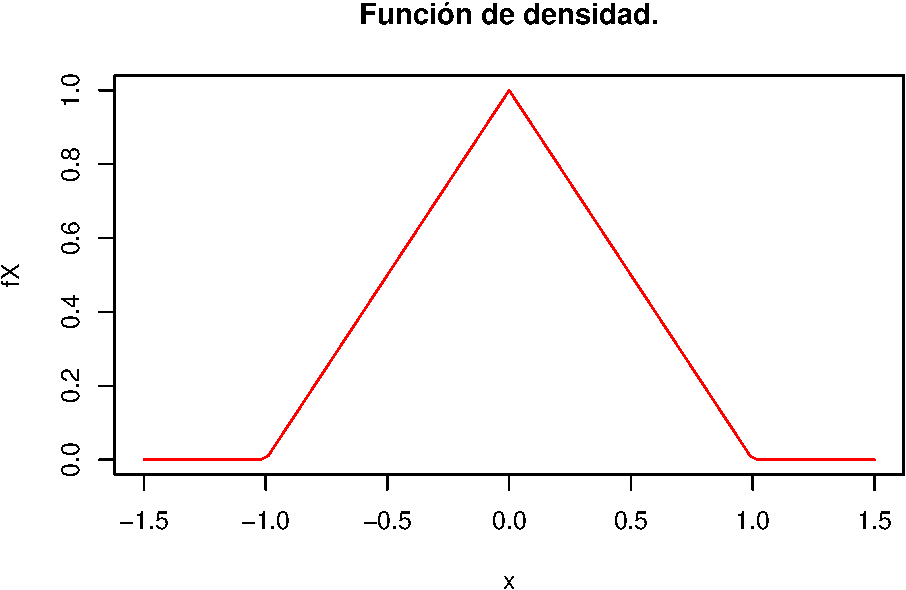
\includegraphics{Tema-2---Variables-Aleatorias_parte2_continuas_Soluciones_files/figure-latex/unnamed-chunk-2-1.pdf}

para calcular la función de distribución hacemos

\begin{eqnarray*}
F_X(x)&=&\int_{-\infty}^t f_X(t)\cdot  dy\\ &=&
\left\{
\begin{array}{ll}
\int_{-\infty}^t 0\cdot dy=0 & \mbox{si } x<-1\\
\int_{-1}^t  1-|t| \cdot dt= \int_{-1}^t  1+t \cdot dt=
\left[t+\frac{t^2}{2}\right]_{t=-1}^{t=x}= & \mbox{si } -1\leq x\leq 0\\ 
\int_{-1}^t  (1-|t|) \cdot dt= \int_{-1}^0  (1+t)\cdot dt+
\int_{0}^x  (1-t) \cdot dt =\frac{1}{2} + 
\left[t-\frac{t^2}{2}\right]_{t=0}^{t=x}, & \mbox{si } -\leq x\leq 0,\\ 
1, & \mbox{si } x\geq 1.
\end{array}\right.
\\
&=& 
\left\{
\begin{array}{ll}
0 & \mbox{si } x\leq -1\\
\left(x+\frac{x^2}{2}\right)- \left(-1+\frac{(-1)^2}{2}\right)=
\left(x+\frac{x^2}{2}\right)+ \frac{1}{2}=\frac{x^2+2\cdot x+1}{2}=
\frac{(x+1)^2}{2} & \mbox{si } -1\leq x\leq 0\\ 
\frac{1}{2}+ \left[\left(x-\frac{x^2}{2}\right)- 0\right]=
\frac{1}{2}+x-\frac{x^2}{2}, & \mbox{si } 0\leq x\leq 1,\\ 
1, & \mbox{si } x\geq 1.
\end{array}\right.
\\
&=&
\left\{
\begin{array}{ll}
0 & \mbox{si } x\leq -1\\
\frac{(x+1)^2}{2}, & \mbox{si } -1\leq x \leq 0,\\ 
\frac{(1-x)^2}{2}, & \mbox{si } 0\leq x\leq 1,\\ 
1, & \mbox{si } x\geq 1.
\end{array}\right.
\end{eqnarray*}

Su gráfica es

\begin{Shaded}
\begin{Highlighting}[]
\NormalTok{FX}\OtherTok{=}\ControlFlowTok{function}\NormalTok{(x)\{}\FunctionTok{sapply}\NormalTok{(x,}
                      \AttributeTok{FUN=}\ControlFlowTok{function}\NormalTok{(x)\{}
\FunctionTok{ifelse}\NormalTok{(x}\SpecialCharTok{\textless{}={-}}\DecValTok{1}\NormalTok{,}\DecValTok{0}\NormalTok{,}\FunctionTok{ifelse}\NormalTok{(x}\SpecialCharTok{\textgreater{}=}\DecValTok{1}\NormalTok{,}\DecValTok{1}\NormalTok{,}\FunctionTok{ifelse}\NormalTok{(x}\SpecialCharTok{\textless{}}\DecValTok{0} \SpecialCharTok{\&}\NormalTok{ x}\SpecialCharTok{\textgreater{}{-}}\DecValTok{1}\NormalTok{, (x}\SpecialCharTok{+}\DecValTok{1}\NormalTok{)}\SpecialCharTok{\^{}}\DecValTok{2}\SpecialCharTok{/}\DecValTok{2}\NormalTok{, }\DecValTok{1}\SpecialCharTok{/}\DecValTok{2}\SpecialCharTok{+}\NormalTok{x}\SpecialCharTok{{-}}\NormalTok{x}\SpecialCharTok{\^{}}\DecValTok{2}\SpecialCharTok{/}\DecValTok{2}\NormalTok{)))  }
\NormalTok{\})}
\NormalTok{\}}

                            
                          
\FunctionTok{FX}\NormalTok{(}\FunctionTok{c}\NormalTok{(}\SpecialCharTok{{-}}\DecValTok{20}\NormalTok{,}\SpecialCharTok{{-}}\DecValTok{1}\NormalTok{,}\SpecialCharTok{{-}}\DecValTok{1}\SpecialCharTok{/}\DecValTok{2}\NormalTok{,}\DecValTok{0}\NormalTok{,}\DecValTok{1}\SpecialCharTok{/}\DecValTok{2}\NormalTok{,}\DecValTok{1}\NormalTok{,}\DecValTok{20}\NormalTok{))}
\end{Highlighting}
\end{Shaded}

\begin{verbatim}
## [1] 0.000 0.000 0.125 0.500 0.875 1.000 1.000
\end{verbatim}

\begin{Shaded}
\begin{Highlighting}[]
\FunctionTok{curve}\NormalTok{(FX,}\AttributeTok{from=}\SpecialCharTok{{-}}\DecValTok{2}\NormalTok{,}\AttributeTok{to=}\DecValTok{2}\NormalTok{,}\AttributeTok{col=}\StringTok{"red"}\NormalTok{,}\AttributeTok{ylab=}\StringTok{"fX"}\NormalTok{,}\AttributeTok{xlab=}\StringTok{"x"}\NormalTok{,}\AttributeTok{main=}\StringTok{"Función de densidad."}\NormalTok{)}
\end{Highlighting}
\end{Shaded}

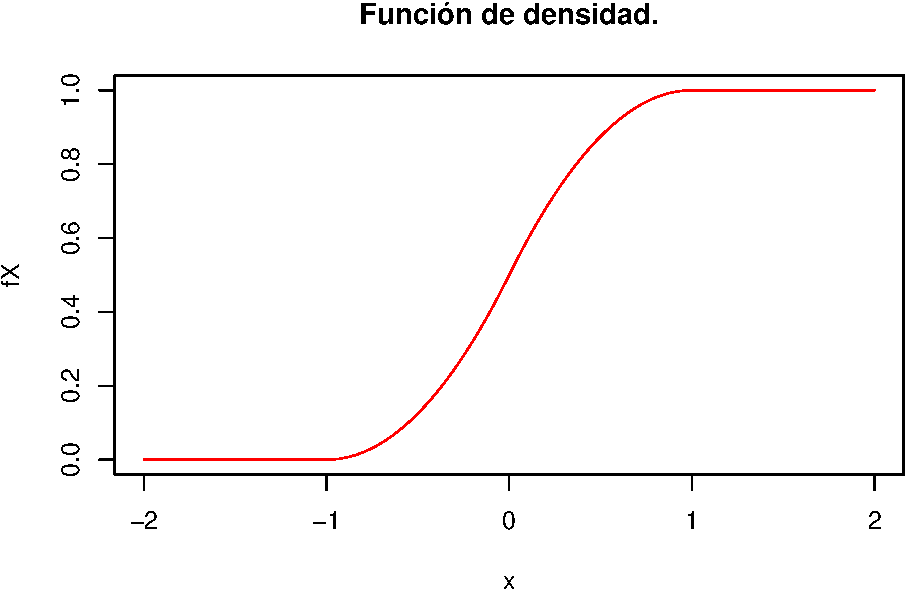
\includegraphics{Tema-2---Variables-Aleatorias_parte2_continuas_Soluciones_files/figure-latex/unnamed-chunk-4-1.pdf}

\hypertarget{problema-5.}{%
\subsection{Problema 5.}\label{problema-5.}}

Hallar la esperanza y la varianza de las variables de los ejercicios
anteriores.

\hypertarget{soluciuxf3n-4}{%
\subsubsection{Solución}\label{soluciuxf3n-4}}

Estas integrales se dejan como ejercicio.

\end{document}
